%%%%%%%%%%%%%%%%%%%%%%%%%%%%%%%%%%%%%%%%%%%%%%%%%%%%%
%   METODOLOGIA
%%%%%%%%%%%%%%%%%%%%%%%%%%%%%%%%%%%%%%%%%%%%%%%%%%%%%

\chapter{Metodologia}

As galáxias com jatos que representam a Categoria 7 (na verdade, para todas as Categorias) foram agrupadas a partir da análise morfológica fornecida na época pelos filmes fotográficos (emulsão IIIa-J de grão fino) da Kodak (Eastman Kodak Company). Portanto, certos detalhes que conseguimos explorar hoje através das imagens de melhor resolução espacial, não foram possíveis nas análises prévias conduzidas por Arp \& Madore. Logo, apenas com as informações presentes nas fotografias para analisar certos níveis de brilho superficial ligeiramente fracos em relação ao esperado, os autores acima poderiam facilmente omitir dados importantes, mesmo para um olho muito bem treinado. Por outro lado, as regiões externas, sendo menos densas e brilhantes, também podiam omitir importantes análises. Como as perturbações podem ter como origem atividades internas, como explosões ou ejeções, ou da interação com objetos vizinhos, fica óbvio pensar que as regiões que circundam as galáxias devem ser também cuidadosamente estudadas. Portanto, uma análise rigorosa das imagens deve ser conduzida no intuito de verificar se de fato o que esta sendo observado é um jato ou alguma outra característica peculiar.

A Categoria 7 contêm um total de 256 galáxias. Porém, antes de lançarmos a análise espectral desse conjunto, elaboramos uma metodologia que objetiva verificar se as galáxias presentes apresentam, de fato, jatos. A metodologia foi adaptada do trabalho sobre o reconhecimento e classificação de galáxias com jatos publicada por Keel \cite{keel1985recognition}. A amostragem final de galáxias será apresentada no próximo Capítulo.

\section{Possíveis Maneiras de Obter um Falso Jato}

\begin{enumerate}
    \item Galáxias Superpostas

Alguns ``jatos`` observados ao longo de nossa linha de visada podem ser, na verdade, puros alinhamentos ocasionais de galáxias, como, por exemplo, o de uma galáxia "face-on" (i.e., de frente) alinhada com o núcleo de uma outra galáxia ``edge-on`` (de perfil). Um exemplo deste efeito é observado na fonte rádio DA 240 \cite{van1983radio} e também na fonte 1240-057 \cite{romanishin19841240}. No óptico, o exemplo bem característico é o da galáxia UGC 3810 (ver Figura \ref{fig:UGC-3810}), onde uma companheira ``edge-on`` superposta foi relacionada de forma errada como um jato na literatura. Apesar da proximidade de ambos objetos, a galáxia ``edge-on`` não apresenta redshift determinado, sendo difícil, portanto, dizer se temos de fato um sistema interagente ou apenas a projeção de uma galáxia no campo.

\begin{figure}[H]
	\centering	
    \caption{UGC 3810}
    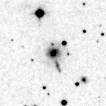
\includegraphics[width=0.7\textwidth]{figuras/ugc3810.jpg}
   	\begin{center}
        \normalsize Fonte: NED-NASA/IPAC \\Este é um claro exemplo de uma superposição entre duas galáxias: uma espital ``face-on`` (centro) e uma outra superposta ``edge-on`` semelhante a um jato (ao Sul). A direção Norte está para cima, e a direção Leste para a esquerda.
    \end{center}
	\label{fig:UGC-3810}
\end{figure}

    \item Efeitos de Maré e Galáxias em Interação

O principal aspecto para a escolha deste item está relacionado à observação de caudas e filamentos projetados, bem retos e estreitos, que podem aparecer como resultado final do efeito de maré em uma galáxia, não sendo, portanto, um jato.
Porém, um aspecto deve ser levado em consideração, pois quando segregamos os efeitos nucleares manifestados através das linhas de emissão presentes em galáxias interagentes (neste caso, via efeito de maré), estamos também excluindo muitos objetos com núcleos ativos que representam potenciais candidatos a jatos, uma vez que a atividade nuclear é catalisada em sistemas que se encontram em interação gravitacional, sendo os jatos os sinais internos desses processos.

Em adição, as interações mais avançadas para o estágio de fusão podem produzir uma série de efeitos quando os sistemas ricos em gás estão envolvidos, e a seleção de estruturas radiais, sem dúvida, produzirá uma fração destes efeitos. Os argumentos dinâmicos baseados no nível de atividade nuclear agora observado podem ser considerados na interpretação dessa característica. Por motivos puramente morfológicos, certos tipos de características de maré podem ser reconhecidos. Sistemas como NGC 1568 (ver Figura \ref{fig:NGC-1568}), com pares de caudas quase simétricas, não são susceptíveis de aparecer como jatos em imagens com resolução suficiente. Leves curvaturas e curvas terminais são mais características dos efeitos de maré do que de jatos.

\begin{figure}[H]
	\centering	
    \caption{NGC 1568}
    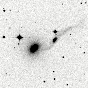
\includegraphics[width=0.7\textwidth]{figuras/ngc1568.jpg}
   	\begin{center}
        \normalsize Fonte: NED-NASA/IPAC \\Exemplo de uma interação gravitacional tipo maré, com a construção de uma cauda como o resultado do processo. A direção Norte está para cima, e a direção Leste para a esquerda.
    \end{center}
	\label{fig:NGC-1568}
\end{figure}

\item Galáxias com Anéis Polares

Esses tipos de sistemas são detectados com maior facilidade quando o disco da galáxia principal é visto quase ao contrário \cite{schweizer1983colliding}, e muitos deles também apresentam anéis externos (perpendiculares) vistos quase de ponta. Os anéis de NGC 4650A (ver Figura \ref{fig:NGC-4650A}), por exemplo, foram de fato originalmente interpretados como pares de jatos (Laustsen e West 1980; Sofue et al., 1982; Mold et al., 1982). No entanto, estes podem ser distinguidos dos jatos verdadeiros pelo fato de serem muitos simétricos sobre o galáxia central. É importante dizer que os jatos ópticos até agora conhecidos são unilaterais ou bastante assimétricos (por exemplo, NGC 1097, para os quais \cite{lorre1978enhancement} relatou relações de brilho de 9:1 e 3:1 para os pares opostos de jatos). Quando não são bastante avançados, os jatos mostram frequentes absorções contra a galáxia central. Vários anéis polares e objetos aparentemente relacionados já foram observados. Algumas pistas morfológicas para a presença de um anel externo e desalinhado requer, muitas vezes, imagens de alta resolução, de modo que a distinção entre anéis e jatos geralmente não é aparente (exceto por considerações de simetria) das fotografias presentes nas placas de céu.

\begin{figure}[H]
	\centering	
    \caption{NGC 4650A}
    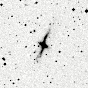
\includegraphics[width=0.7\textwidth]{figuras/ngc4650A.jpg}
   	\begin{center}
        \normalsize Fonte: NED-NASA/IPAC \\Exemplo de um anel polar que pode dar a falsa impressão de um jato. A direção Norte está para cima, e a direção Leste para a esquerda.
    \end{center}
	\label{fig:NGC-4650A}
\end{figure}

\item Distribuições de Luz Assimétrica em Galáxias de Perfil (Edge-on)

Sabemos que a poeira presente ao longo dos braços de galáxias espirais produz uma forte assimetria na aparência destes objetos quando visto ao longo de seu plano \cite{de1958tilt}. Fisicamente, isso significa que o lado que se aproxima do disco é mais brilhante do que o lado que se afasta. Esse contraste pode ser tão extremo quanto a aparência de um jato ao longo da
eixo principal, como visto, por exemplo, na galáxia Arp 207 (Figura \ref{fig:ARP-207}).

\begin{figure}[H]
	\centering	
    \caption{ARP 207}
    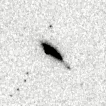
\includegraphics[width=0.7\textwidth]{figuras/arp207.jpg}
   	\begin{center}
        \normalsize Fonte: NED-NASA/IPAC \\Contraste observado que pode revelar a presença de um falso jato. A direção Norte está para cima, e a direção Leste para a esquerda.
    \end{center}
	\label{fig:ARP-207}
\end{figure}


\item Galáxias com Sistemas de Filamentos Ópticos

São conhecidos vários tipos de sistemas de filamentos extensivos (linha de emissão) que ocorrem em torno de galáxias, algumas das quais apresentam características que imitam a aparência de jatos. Uma série de galáxias em aglomerados centrais apresentam filamentos de linha de emissão aparentemente associados a fluxos de acréscimo (por exemplo, \cite{heckman1981optical}). Algumas dessas características vistas individualmente, especialmente aquelas em torno de NGC 1275 (ver Figura \ref{fig:1275}), poderiam aparecer como jatos. Estudos espectroscópicos sugerem que os filamentos estão caindo na galáxia \cite{keel1985recognition}. Portanto, muitos jatos ou uma aparência filamentar devem ser excluídos das pesquisas de jatos ópticos.

\begin{figure}[H]
	\centering	
    \caption{NGC 1275}
    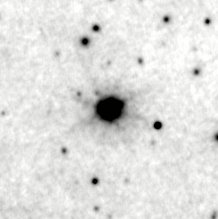
\includegraphics[width=0.7\textwidth]{figuras/ngc1275.jpg}
   	\begin{center}
        \normalsize Fonte: NED-NASA/IPAC \\Sistema de filamentos característicos de linhas de emissão também podem dar a falsa impressão de jatos. A direção Norte está para cima, e a direção Leste para a esquerda.
    \end{center}
	\label{fig:1275}
\end{figure}

\item Barras Galácticas Normais

Ocasionalmente, especialmente no catálogo Zwicky de galáxias e aglomerados \url{(ftp://cdsarc.u-strasbg.fr/cats/VII/190/)}, os objetos são listados como jatos que parecem ser, em uma inspeção mais direta, barras bastante comuns em discos fracos. Um exemplo é a galácia UGC 01198 (VII Zw 3), ver Figura \ref{fig:sugc01198}. Portanto, esses tipos de galáxias podem ser eliminadas das pesquisas rejeitando pares com características brilhantes e simétricas, como no caso de anéis polares.

\begin{figure}[H]
	\centering	
    \caption{ugc01198}
    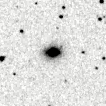
\includegraphics[width=0.7\textwidth]{figuras/ugc01198.jpg}
   	\begin{center}
        \normalsize Fonte: NED-NASA/IPAC \\Barras em galáxias normais representam também uma fonte comum para caracterizar jatos. A direção Norte está para cima, e a direção Leste para a esquerda.
    \end{center}
	\label{fig:sugc01198}
\end{figure}

\item Galáxias com Hastes

O astrônomo russo Vorontsov-Velyaminov em dois artigos publicados em 1959 e 1977, chamou a atenção para sistemas que apresentam conexões relativamente curtas que podem ocorrer dentro de um intervalo morfológico. Estas, por sua vez, estão associadas a formação de estrelas ativas, podendo ser o resultado de sua propagação em um disco externo. Como exemplo, o disco interno e as partes externas da NGC 573 são mostrados na Figura \ref{fig:ngc573}. As regiões internas mostram uma estrutura espiral clara. Espectros revelam linhas de emissão nuclear indicativas da formação de estrelas. Como as hastes não chegam muito para o núcleo, elas são características mais prováveis de origem local do que nuclear.

\begin{figure}[H]
	\centering	
    \caption{ngc573}
    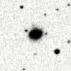
\includegraphics[width=0.7\textwidth]{figuras/ngc573.jpg}
   	\begin{center}
        \normalsize Fonte: NED-NASA/IPAC \\Exemplo de uma galáxia onde a formação de hastes podem levar a compreensão de jatos. A direção Norte está para cima, e a direção Leste para a esquerda.
    \end{center}
	\label{fig:ngc573}
\end{figure}

\item Estrelas Superpostas

Este é um típico caso onde estrelas projetadas contra o fundo de um halo galáctico podem produzir alguns efeitos, inclusive, os de jatos em certos objetos. No entanto, é importante ressaltar que alguns jatos síncrotrons estão fortemente dominados por regiões relativamente pequenas que parecem estelares em redshifts maiores do que 0,10. Por exemplo, o objeto localizado perto da galáxia  Fairall 71 (ver Figura \ref{fig:071}) interpretado como um jato de luz síncrotron (por Fricke, Kollatschny e Loose (1984)) é de aparência estelar. Por outro lado, o jato detectado em M87 e por pequenas regiões (condensações) que, a uma distância correspondente a z $\sim$ 0,05, não seria resolvido a partir do solo. As galáxias compactas também podem produzir efeitos bem como os das estrelas. 

\begin{figure}[H]
	\centering	
    \caption{Fairall 071}
    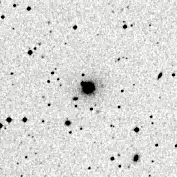
\includegraphics[width=0.7\textwidth]{figuras/fairall071.jpg}
   	\begin{center}
        \normalsize Fonte: NED-NASA/IPAC \\Estrelas projetadas próximas ao campo podem produzir efeitos característicos de jatos. A direção Norte está para cima, e a direção Leste para a esquerda.
    \end{center}
	\label{fig:071}
\end{figure}

\item Artefatos Fotográficos

Este é um exemplo associado com os níveis de contraste, geralmente muito baixos em relação ao nível de fundo, onde os grãos de alguns tipos de emulsões fotográficas exibem. Por exemplo, a maioria dos candidatos de jatos relacionados por Vorontsov-Velyaminov (1966,1972) aparecem a partir da inspeção das placas fotográficas do Sky Survey, cujo brilho superficial é muito fraco. Características muito fracas, a menos que sejam bem grandes, devem, portanto, ser confirmadas em materiais de melhor resolução espacial. Alguns controles sobre este efeito podem ser exercidos observando o nível no qual as caudas não conectadas a qualquer coisa começam a aparecer na placa fotográfica. A combinação aleatória de um amontoado de grandes grãos e do gradiente de exposição acentuado presente em um envelope de galáxia, pode ser particularmente atraente e produzir uma imagem de jato muito convincente. Esse aspecto pode ser ilustrado na galáxia UGC 1378 (Figura \ref{fig:1378}). 

\begin{figure}[H]
	\centering	
    \caption{UGC 1378}
    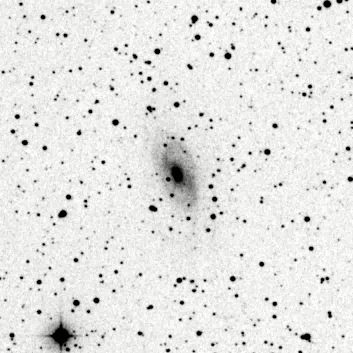
\includegraphics[width=0.7\textwidth]{figuras/ugc1378.jpg}
   	\begin{center}
        \normalsize Fonte: NED-NASA/IPAC \\Emulsões fotográficas de baixa razão sinal-ruído podem produzir artefatos nas imagens semelhantes a jatos. A direção Norte está para cima, e a direção Leste para a esquerda.
    \end{center}
	\label{fig:1378}
\end{figure}

\item Galáxias com Estruturas Caóticas

De um modo simples, os jatos são, obviamente, mais fáceis de serem percebidos contra o fundo liso e regular de uma galáxia elíptica. Em espirais do tipo morfológico de Hubble intermediário ou tardio, a estrutura interna pode ser tão complexa ou desorganizada que os alinhamentos radiais de condensações são improváveis. Portanto, existem certos compromissos subjetivos a serem feitos na seleção de candidatos de jatos entre galáxias de tipo tardio. Existem dicas claras sobre a possível presença de um jato quando o material se estende para fora da estrutura galáctica visível ou aponta para um núcleo ativo. Os sistemas irregulares podem exibir uma estrutura semelhante a um jato, talvez produzida pela formação de estrelas de propagação. NGC 1602 é um exemplo deste cenário (Figura \ref{fig:1602}).

\begin{figure}[H]
	\centering	
    \caption{NGC 1602}
    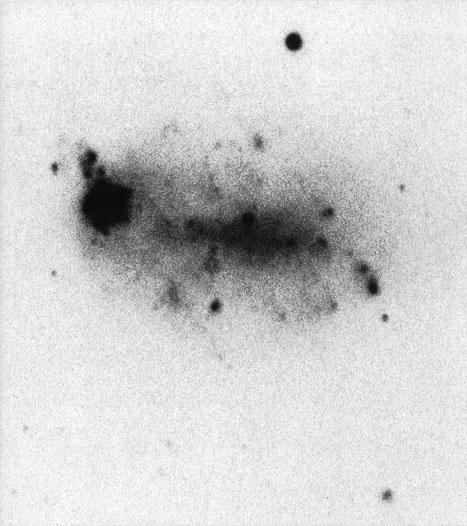
\includegraphics[width=0.7\textwidth]{figuras/ngc1602.jpg}
   	\begin{center}
        \normalsize Fonte: NED-NASA/IPAC \\Determinadas estruturas produzidas por condensações internas podem levar a intrepretação de falsos jatos. A direção Norte está para cima, e a direção Leste para a esquerda.
    \end{center}
	\label{fig:1602}
\end{figure}

\end{enumerate}

\section{Critérios Adicionais de Seleção}

 Além das descrições acima que ilustram algumas das possíveis maneiras de gerar um falso jato, também incluímos os seguintes critérios neste trabalho para excluir possíveis galáxias que apresentam falsos jatos:

\begin{enumerate}
    
\item Os verdadeiros jatos não devem apresentam mais do que alguns por cento da luminosidade óptica das galáxias hospedeiras. O valor de referência foi estabelecido em 0,03 (de acordo com \cite{keel1985recognition}). No entanto, para quantificar essa análise nas galáxias estudadas, valores para a razão de luminosidade foram obtidas diretamente da banda B, a qual possibilita uma análise dos componentes de maior energia.

\item Presença de jatos unilaterais ou muito assimétricos em intensidade óptica. 

\item Possíveis extensões unilaterais ao longo dos principais eixos das
galáxias (a: semi-eixo maior, e b: semi-eixo menor) com alto valor de inclinação (i = cos (b/a)) são susceptíveis de serem braços espirais.

\item Comparação do jato com a vizinhança próxima e o fundo do céu.

\item Com resolução angular suficiente para realizar uma medida, é possível obter uma proporção de 8:1\cite{keel1985recognition} para separar jatos e outros objetos.

\end{enumerate}

Desse modo, a partir dos aspectos apresentados acima que caracterizam algumas possíveis formas e maneiras de gerar um falso jato, submetemos a uma análise visual as 256 galáxias peculiares extraídas de diferentes bancos de dados e bandas espectrais: SDSS (B), 2MASS (vermelho, J; poeira, K), WISE (infra- vermelho, 3.4 e 22$\mu$m), e GALEX (ultravioleta próximo). Após uma análise sobre esse conjunto, 7 galáxias (cerca de 3\%) foram então separadas para uma análise mais criteriosa, com o intuito de alocá-las (ou não) em alguma outra Categoria (15, por exemplo) do Catálogo de Arp \& Madore. Das 249 galáxias selecionadas, foi possível extrair informações fotométricas de 201 (ver Apêndice A). Dessas, 125 apresentam espectros ópticos na literatura, as quais foram agrupadas em grupos de galáxias normais (52) e ativas (73), Apêndices B e C, respectivamente. Portanto, essa foi a seleção dos objetos que passaremos a realizar a modelagem com o código de síntese espectral STARLIGHT \cite{cid2004star,fernandes2005semi,asari2007history}. Uma descrição da base de dados empregada nesse trabalho é apresentada no Capítulo seguinte.